\documentclass[tikz,border=4pt,11pt]{standalone}
\usepackage{amsmath}
\definecolor{ink}{RGB}{42,52,64}
% The fourteen Dyck paths of semilength four, labelled by their area
% sequences (the heights before the up-steps), in lexicographic order.
% Generated from the area sequences; each path is drawn with up and down steps.
\begin{document}
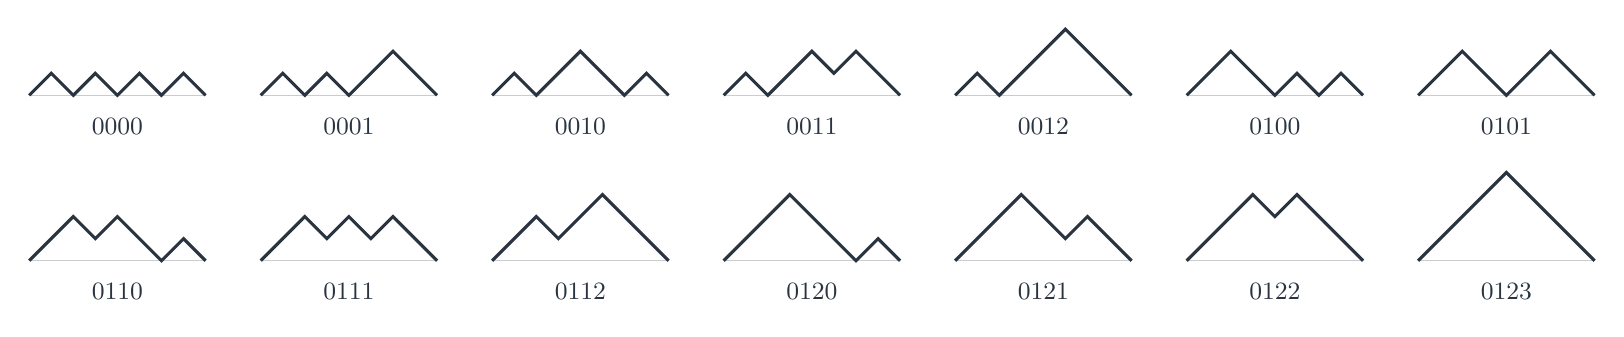
\begin{tikzpicture}[x=.28cm,y=.28cm,text=ink]
  \begin{scope}[shift={(0.0,0.0)}]
    \draw[ink!25] (0,0) -- (8,0);
    \draw[ink,line width=1.1pt] (0,0) -- (1,1) -- (2,0) -- (3,1) -- (4,0) -- (5,1) -- (6,0) -- (7,1) -- (8,0);
    \node[font=\small] at (4,-1.4) {$0000$};
  \end{scope}
  \begin{scope}[shift={(10.5,0.0)}]
    \draw[ink!25] (0,0) -- (8,0);
    \draw[ink,line width=1.1pt] (0,0) -- (1,1) -- (2,0) -- (3,1) -- (4,0) -- (5,1) -- (6,2) -- (7,1) -- (8,0);
    \node[font=\small] at (4,-1.4) {$0001$};
  \end{scope}
  \begin{scope}[shift={(21.0,0.0)}]
    \draw[ink!25] (0,0) -- (8,0);
    \draw[ink,line width=1.1pt] (0,0) -- (1,1) -- (2,0) -- (3,1) -- (4,2) -- (5,1) -- (6,0) -- (7,1) -- (8,0);
    \node[font=\small] at (4,-1.4) {$0010$};
  \end{scope}
  \begin{scope}[shift={(31.5,0.0)}]
    \draw[ink!25] (0,0) -- (8,0);
    \draw[ink,line width=1.1pt] (0,0) -- (1,1) -- (2,0) -- (3,1) -- (4,2) -- (5,1) -- (6,2) -- (7,1) -- (8,0);
    \node[font=\small] at (4,-1.4) {$0011$};
  \end{scope}
  \begin{scope}[shift={(42.0,0.0)}]
    \draw[ink!25] (0,0) -- (8,0);
    \draw[ink,line width=1.1pt] (0,0) -- (1,1) -- (2,0) -- (3,1) -- (4,2) -- (5,3) -- (6,2) -- (7,1) -- (8,0);
    \node[font=\small] at (4,-1.4) {$0012$};
  \end{scope}
  \begin{scope}[shift={(52.5,0.0)}]
    \draw[ink!25] (0,0) -- (8,0);
    \draw[ink,line width=1.1pt] (0,0) -- (1,1) -- (2,2) -- (3,1) -- (4,0) -- (5,1) -- (6,0) -- (7,1) -- (8,0);
    \node[font=\small] at (4,-1.4) {$0100$};
  \end{scope}
  \begin{scope}[shift={(63.0,0.0)}]
    \draw[ink!25] (0,0) -- (8,0);
    \draw[ink,line width=1.1pt] (0,0) -- (1,1) -- (2,2) -- (3,1) -- (4,0) -- (5,1) -- (6,2) -- (7,1) -- (8,0);
    \node[font=\small] at (4,-1.4) {$0101$};
  \end{scope}
  \begin{scope}[shift={(0.0,-7.5)}]
    \draw[ink!25] (0,0) -- (8,0);
    \draw[ink,line width=1.1pt] (0,0) -- (1,1) -- (2,2) -- (3,1) -- (4,2) -- (5,1) -- (6,0) -- (7,1) -- (8,0);
    \node[font=\small] at (4,-1.4) {$0110$};
  \end{scope}
  \begin{scope}[shift={(10.5,-7.5)}]
    \draw[ink!25] (0,0) -- (8,0);
    \draw[ink,line width=1.1pt] (0,0) -- (1,1) -- (2,2) -- (3,1) -- (4,2) -- (5,1) -- (6,2) -- (7,1) -- (8,0);
    \node[font=\small] at (4,-1.4) {$0111$};
  \end{scope}
  \begin{scope}[shift={(21.0,-7.5)}]
    \draw[ink!25] (0,0) -- (8,0);
    \draw[ink,line width=1.1pt] (0,0) -- (1,1) -- (2,2) -- (3,1) -- (4,2) -- (5,3) -- (6,2) -- (7,1) -- (8,0);
    \node[font=\small] at (4,-1.4) {$0112$};
  \end{scope}
  \begin{scope}[shift={(31.5,-7.5)}]
    \draw[ink!25] (0,0) -- (8,0);
    \draw[ink,line width=1.1pt] (0,0) -- (1,1) -- (2,2) -- (3,3) -- (4,2) -- (5,1) -- (6,0) -- (7,1) -- (8,0);
    \node[font=\small] at (4,-1.4) {$0120$};
  \end{scope}
  \begin{scope}[shift={(42.0,-7.5)}]
    \draw[ink!25] (0,0) -- (8,0);
    \draw[ink,line width=1.1pt] (0,0) -- (1,1) -- (2,2) -- (3,3) -- (4,2) -- (5,1) -- (6,2) -- (7,1) -- (8,0);
    \node[font=\small] at (4,-1.4) {$0121$};
  \end{scope}
  \begin{scope}[shift={(52.5,-7.5)}]
    \draw[ink!25] (0,0) -- (8,0);
    \draw[ink,line width=1.1pt] (0,0) -- (1,1) -- (2,2) -- (3,3) -- (4,2) -- (5,3) -- (6,2) -- (7,1) -- (8,0);
    \node[font=\small] at (4,-1.4) {$0122$};
  \end{scope}
  \begin{scope}[shift={(63.0,-7.5)}]
    \draw[ink!25] (0,0) -- (8,0);
    \draw[ink,line width=1.1pt] (0,0) -- (1,1) -- (2,2) -- (3,3) -- (4,4) -- (5,3) -- (6,2) -- (7,1) -- (8,0);
    \node[font=\small] at (4,-1.4) {$0123$};
  \end{scope}
\end{tikzpicture}
\end{document}
